

\chapter{System Design}

This chapter outlines the chosen methodology for the UAV navigation system, detailing the pipeline and its various components. The system is designed to accurately estimate the UAV's position and heading, even in scenarios where GPS data is unreliable or unavailable. The high-level flow of the system is illustrated in Figure \ref{fig:HighLevelFlow}.

\begin{figure}[H]
    \centering
    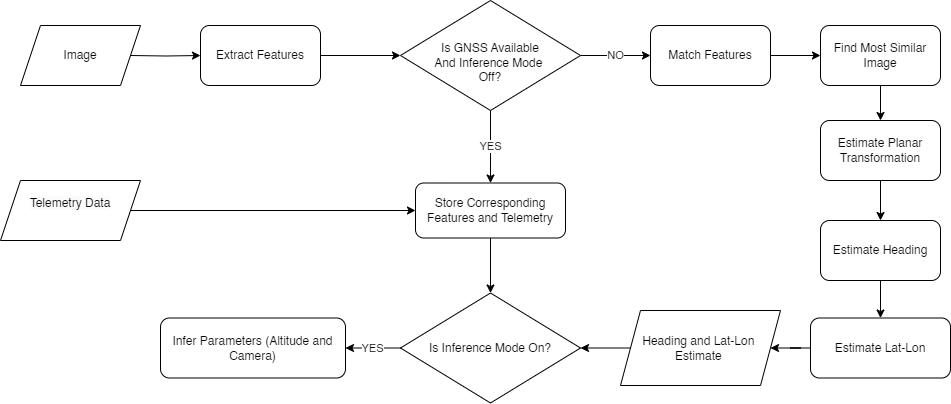
\includegraphics[width=0.8\textwidth]{Chapter 3/Chap3Figs/HighLevelFlow.png}
    \caption{High-Level Flow of the System}
    \label{fig:HighLevelFlow}
\end{figure}



\section{System Pipeline}

The UAV image-processing pipeline comprises several stages, each addressing specific goals in the larger aim to estimate the new GPS and heading of the UAV. These stages require varying levels of precision and efficiency to ensure robust performance.

\subsection{Pipeline Stages}

\begin{enumerate}
    \item \textbf{Image Input:}  
    The process begins with capturing a live image from the UAV’s downward-facing camera. This real-time visual input provides essential information about the UAV’s environment, forming the basis for position estimation.

    \item \textbf{Feature Extraction:}  
    Keypoints and descriptors are extracted from the current image to aid in the matching process. This extraction occurs in two layers:
    \begin{enumerate}
        \item \textbf{Coarse Layer:} Used for proximity search space reduction.
        \item \textbf{Dense Layer:} Used for precise matching and transformation estimation. 
    \end{enumerate}
    By also performing feature extraction when GPS is available, the system reduces computational load during the critical phase when GPS is lost.

    \item \textbf{Storage (Telemetry and Features):}  
    Extracted features (keypoints and descriptors) along with telemetry data (GPS position and heading) are stored for future reference. Stored features facilitate relative transformation inference when GPS is unavailable, while telemetry data assists in converting relative transformations to real-world coordinates and headings.

    \item \textbf{Match Features:}  
    Features between the current image and reference images are matched to ensure that comparisons are based on mutual features. This involves two matching stages:
    \begin{enumerate}
        \item \textbf{Coarse Matching:} Matches the coarse layer of features to reduce the search space.
        \item \textbf{Dense Matching:} Matches the dense layer for precise position estimation.
    \end{enumerate}

    \item \textbf{Similarity Comparison:}  
    The system compares the input image with reference images to identify the most similar one. This comparison is conducted using global matching techniques on aligned images to ensure efficiency and accuracy.
    \begin{enumerate}
        \item \textbf{Proximity Search Space Reduction:}  
        Reduces the search space based on proximity from the last known or estimated GPS location. A dynamic search radius is employed, expanding until five potential matches are found to balance computational efficiency and robustness against expected location deviations.
        
        \item \textbf{Rotational Alignment:}  
        Estimates the rotation between the input and reference images using the coarse layer of features. The images are aligned using the course estimate as global matchers tolerate minor rotational inaccuracies well.
        
        \item \textbf{Best Match Identification:}  
        Computes similarity scores between the input image and each candidate image using global matching techniques. The image with the highest similarity score is selected as the best match, serving as the reference for position estimation.
    \end{enumerate}



    \item \textbf{Planar Transformation Estimation:}  
    After identifying the best match, the system performs a precise estimation of both rotation and translation between the input and reference images using the dense match layer. This involves several sub-steps to enhance accuracy:
    \begin{enumerate}
        \item \textbf{Angle Estimation:}  
        Utilizes the chosen transformation method to obtain a precise estimate of the rotation between the input and reference images, forming the basis for heading estimation.
        
        \item \textbf{Image Alignment \& Recomputation of Dense Layer:}  
        Aligns the input image with the reference image based on the estimated rotation, thereby removing non-mutual information by rotating it off the canvas. The dense layer of features is recomputed on the aligned images to ensure accurate translation estimates.
        
        \item \textbf{Translation Estimate:}  
        Performs a precise estimation of translation between the two images using the refined dense layer, providing the basis for GPS inference.
    \end{enumerate}

    \item \textbf{Update to Global Coordinate System:}  
    The estimated translation, initially in the internal image coordinate system (pixels), must be converted to real-world coordinates (metres) and then to the global coordinate system (longitude and latitude). This conversion involves several stages:
    \begin{enumerate}
        \item \textbf{Heading Update:}  
        Adds the estimated rotation to the reference image's heading to determine the UAV's new heading.
        
        \item \textbf{Translation Rotation from Internal to Global Coordinate System:}  
        Rotates the translation vector by the UAV's estimated global heading to align it with the global coordinate system without altering its magnitude.
        
        \item \textbf{Pixel to Metres (Relative):}  
        Converts the estimated change in pixels to metres using the dynamically inferred conversion factor. 
        
        \item \textbf{Metres to Global Coordinate System (Relative):}  
        Translates the metre-based changes to relative changes in longitude and latitude using the following equations:
        \begin{equation}
            \Delta \text{Longitude} = \frac{\Delta \text{Metres}}{111320 \times \cos(\text{Latitude})}
        \end{equation}
        \begin{equation}
            \Delta \text{Latitude} = \frac{\Delta \text{Metres}}{111320}
        \end{equation}
        These calculations account for the Earth's oblate spheroid shape, ensuring accurate positional data by adjusting for the decreasing distance between longitudes as one moves towards the poles.
        
        \item \textbf{Conversion to Absolute GPS:}  
        Adds the relative changes in longitude and latitude to the GPS coordinates of the reference image, resulting in the UAV's new GPS position.
    \end{enumerate}

    \item \textbf{Output New GPS and Heading:}  
    The calculated translation and rotation values are used to estimate the UAV's new GPS coordinates and heading. This enables pilots to navigate the UAV back to its base along the original path, even in the absence of GPS.

    \item \textbf{Dynamic Parameter Inference:}  
    This stage is performed while GPS is available. It estimates the GPS position using a temporary pixel-to-metre conversion factor of 1, utilizing the pipeline's stages to compute this estimate. The estimated GPS is compared to the ground truth GPS, and the difference is used to adjust the pixel-to-metre conversion factor. This ensures accurate conversion across datasets with varying altitudes. The first five images are used to infer this scaling factor.


\end{enumerate}



\section{Conclusion}

The system design integrates feature extraction, matching, and transformation estimation to enable precise UAV navigation, even in the absence of reliable GPS data. By employing a combination of diverse feature detectors and optimizing various pipeline stages, the system ensures robustness, accuracy, and computational efficiency across different operational scenarios. 

